\chapter{考察}
\label{ch:discussion}
\ref{ch:discussion}章では\ref{ch:results}章での結果との比較とを行う。
\ref{sec:comparison_sofie}節では、ノルウェー・トロムソにおける解析結果(\ref{sec:results_tromsoe}節)において、SOFIE: Solar Occultation for Ice Experiment(詳細は付録\ref{app:sofie})によって観測データを用いた比較を行う。
\ref{sec:comparison_eep}節では、POES/MetOp: Polar Orbiting Environmental Satellites/Meteorological Operational Satellite(詳細は付録\ref{app:poes})衛星の観測によるデータおよびNASAが提供しているOMNI Web Dataを用いて比較を行う。


\section{SOFIEデータによって導出されたNO柱密度との比較}
\label{sec:comparison_sofie}
まずは、ミリ波分光計を用いた\ce{NO}の観測データの妥当性を確認するため、SOFIEによる\ce{NO}の高度プロファイルデータを用いた。
今回、トロムソの柱密度を導出した期間と同じ時期にトロムソ付近の緯度(およそ65 - 80\textdegree Nの範囲)で観測されたSOFIEのデータを用いた。
その比較結果を図\ref{fig:sofie_mmcd}に示す。
\begin{figure}[htbp]
    \centering
    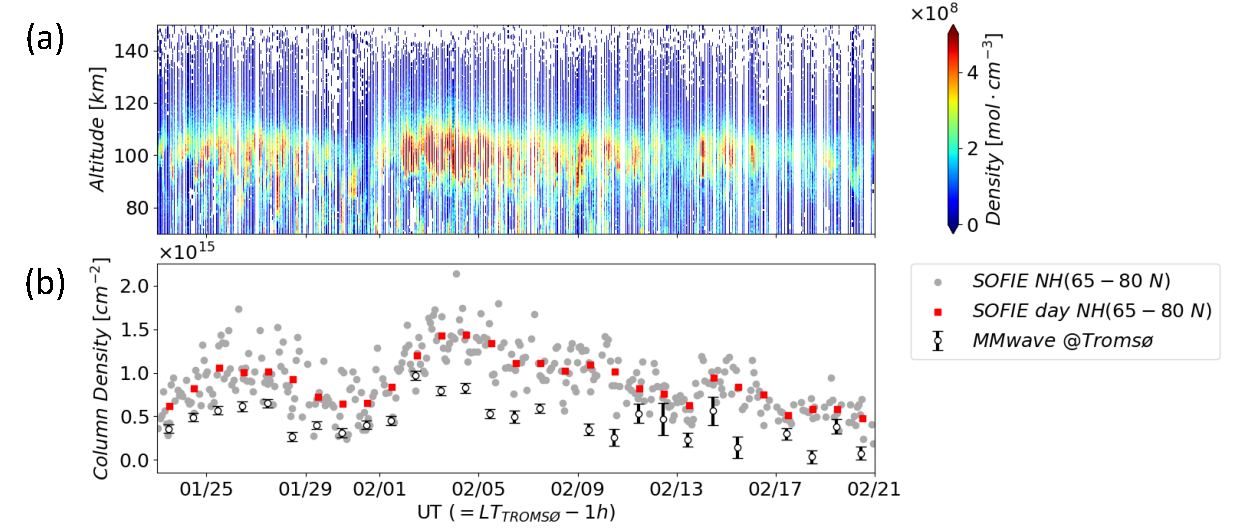
\includegraphics[width=\linewidth]{master_thesis_contents/master_thesis_fig/sofie_mmcd.pdf}
    \caption{(a)SOFIEのNO高度プロファイルデータおよび(b)ミリ波分光計を用いて導出したトロムソの柱密度とSOFIEの高度プロファイルデータから導出した柱密度の比較(エラーバー付きのプロットがミリ波データから導出した柱密度、グレーの丸形プロットがSOFIEの高度プロファイルデータから導出した柱密度、赤色の四角プロットが1日平均したSOFIEの柱密度)}
    \label{fig:sofie_mmcd}
\end{figure}



\section{高エネルギー電子の降り込みとの比較}
\label{sec:comparison_eep}
電子フラックス

% \begin{figure}[htbp]
%     \centering
%     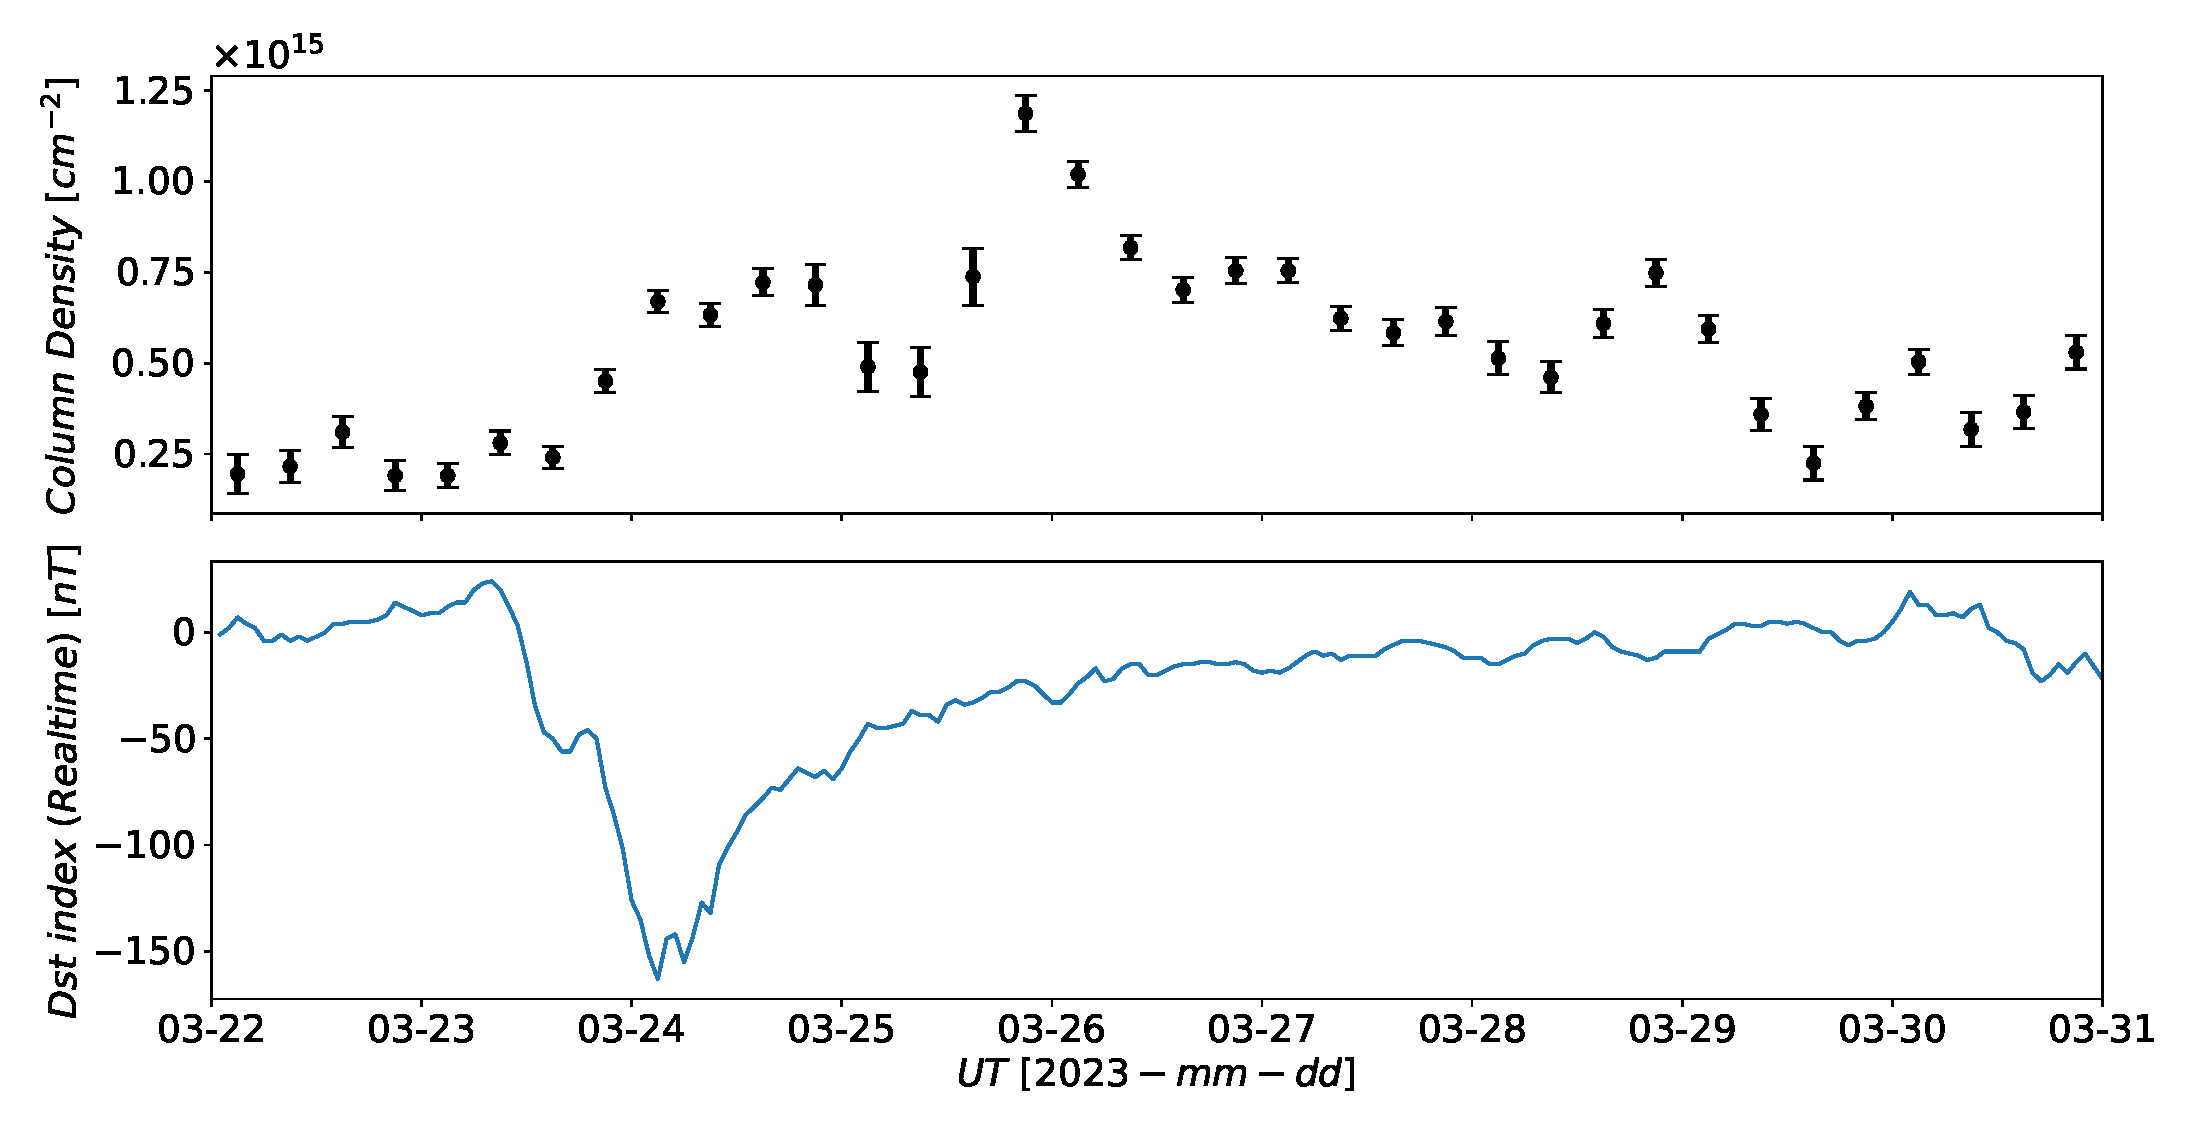
\includegraphics[width=\linewidth]{master_thesis_contents/master_thesis_fig/column_density_spectr6_dst_syowa.pdf}
%     \caption{昭和基地における柱密度(1段目。図\ref{fig:column_density_spectr6_syowa}と同じ)とDst指数(2段目)との比較}
%     \label{fig:dst_mmcd_syowa}
% \end{figure}
% Dst指数のグラフ
\begin{figure}[htbp]
    \centering
    \begin{minipage}{\linewidth}
        \centering
        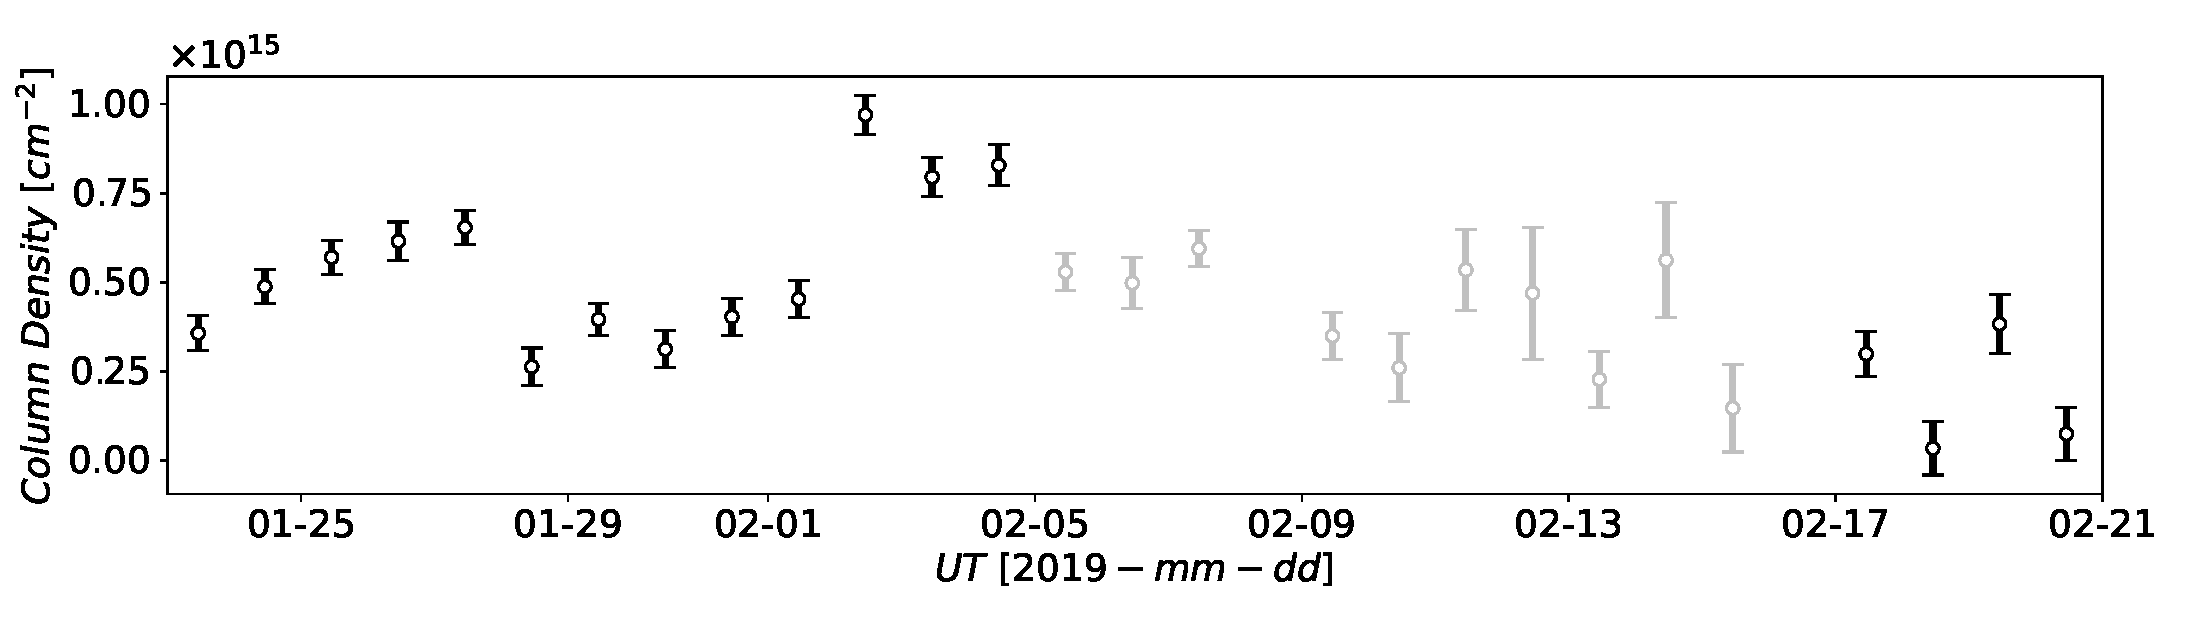
\includegraphics[width=\linewidth]{master_thesis_contents/master_thesis_fig/avg_ColumnDensity_tromsoe.pdf}
    \end{minipage}
    \begin{minipage}{\linewidth}
        \centering
        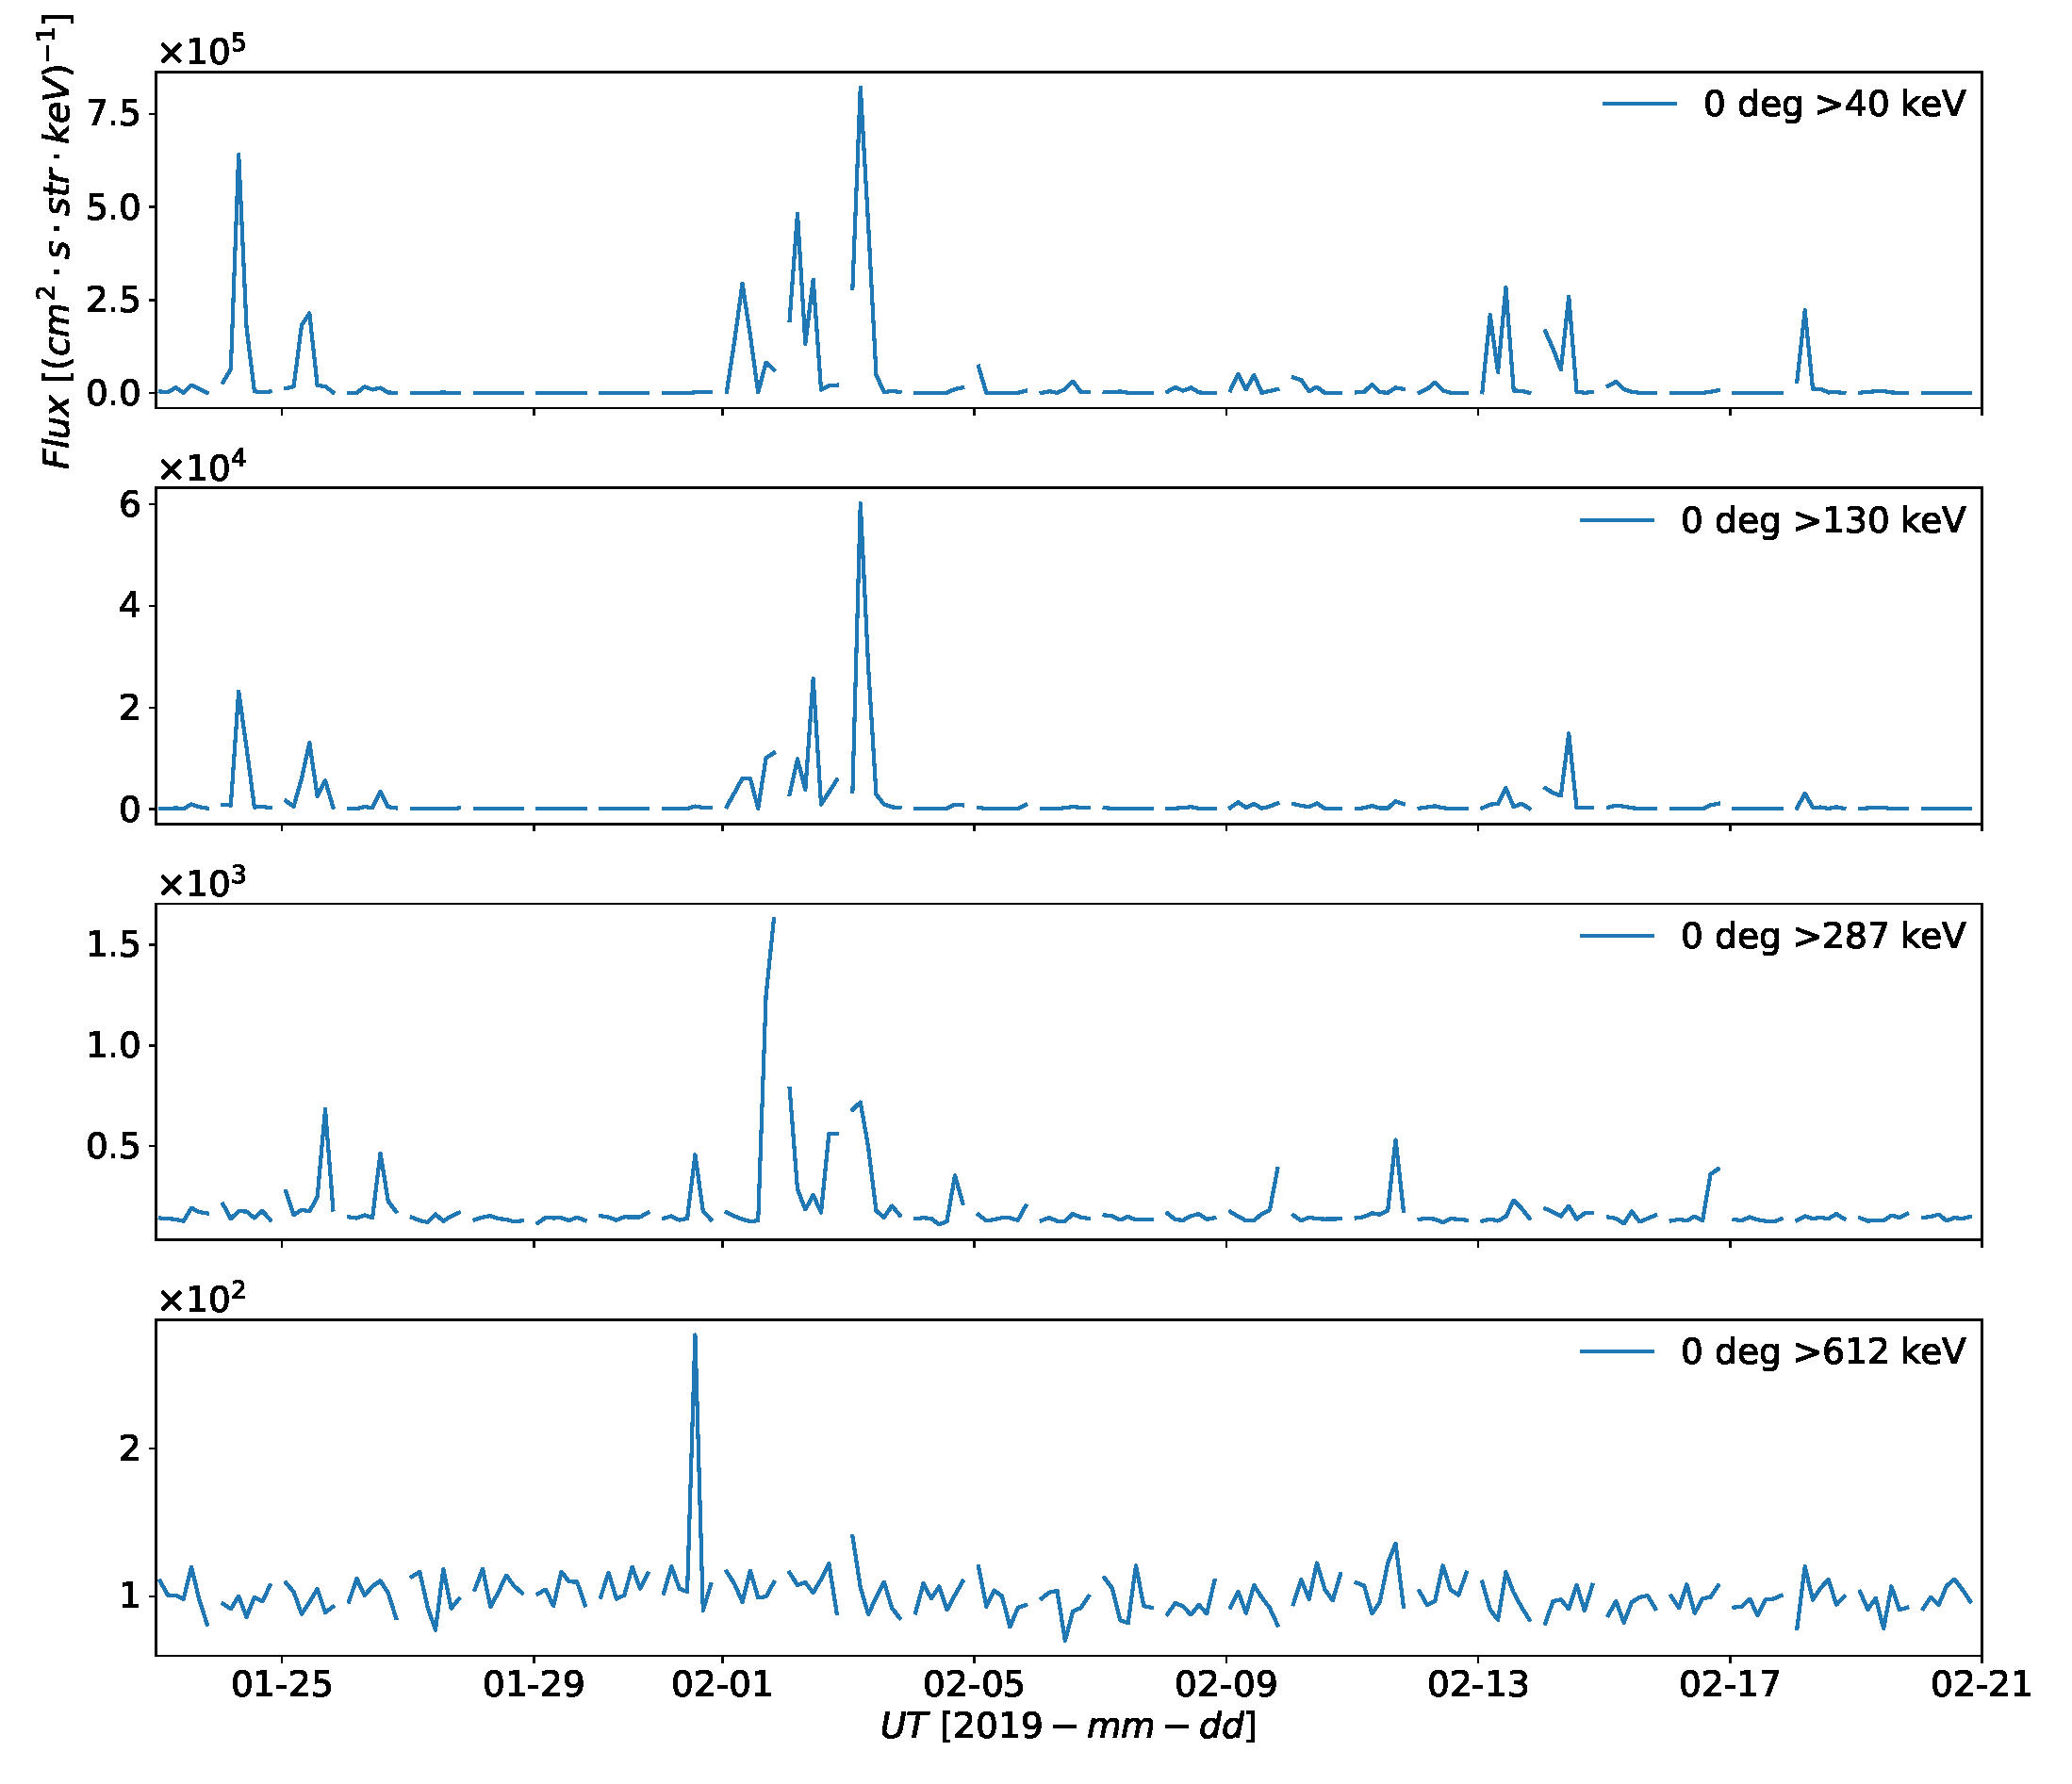
\includegraphics[width=\linewidth]{master_thesis_contents/master_thesis_fig/poes_tromsoe_0deg.pdf}
    \end{minipage}
    \caption{トロムソにおける柱密度(1段目。図\ref{fig:avg_ColumnDensity_tromsoe}と同じ)と電子フラックスデータ(2-5段目)との比較}
    \label{fig:ele_mmcd_tromsoe}
\end{figure}
\begin{figure}[htbp]
    \centering
    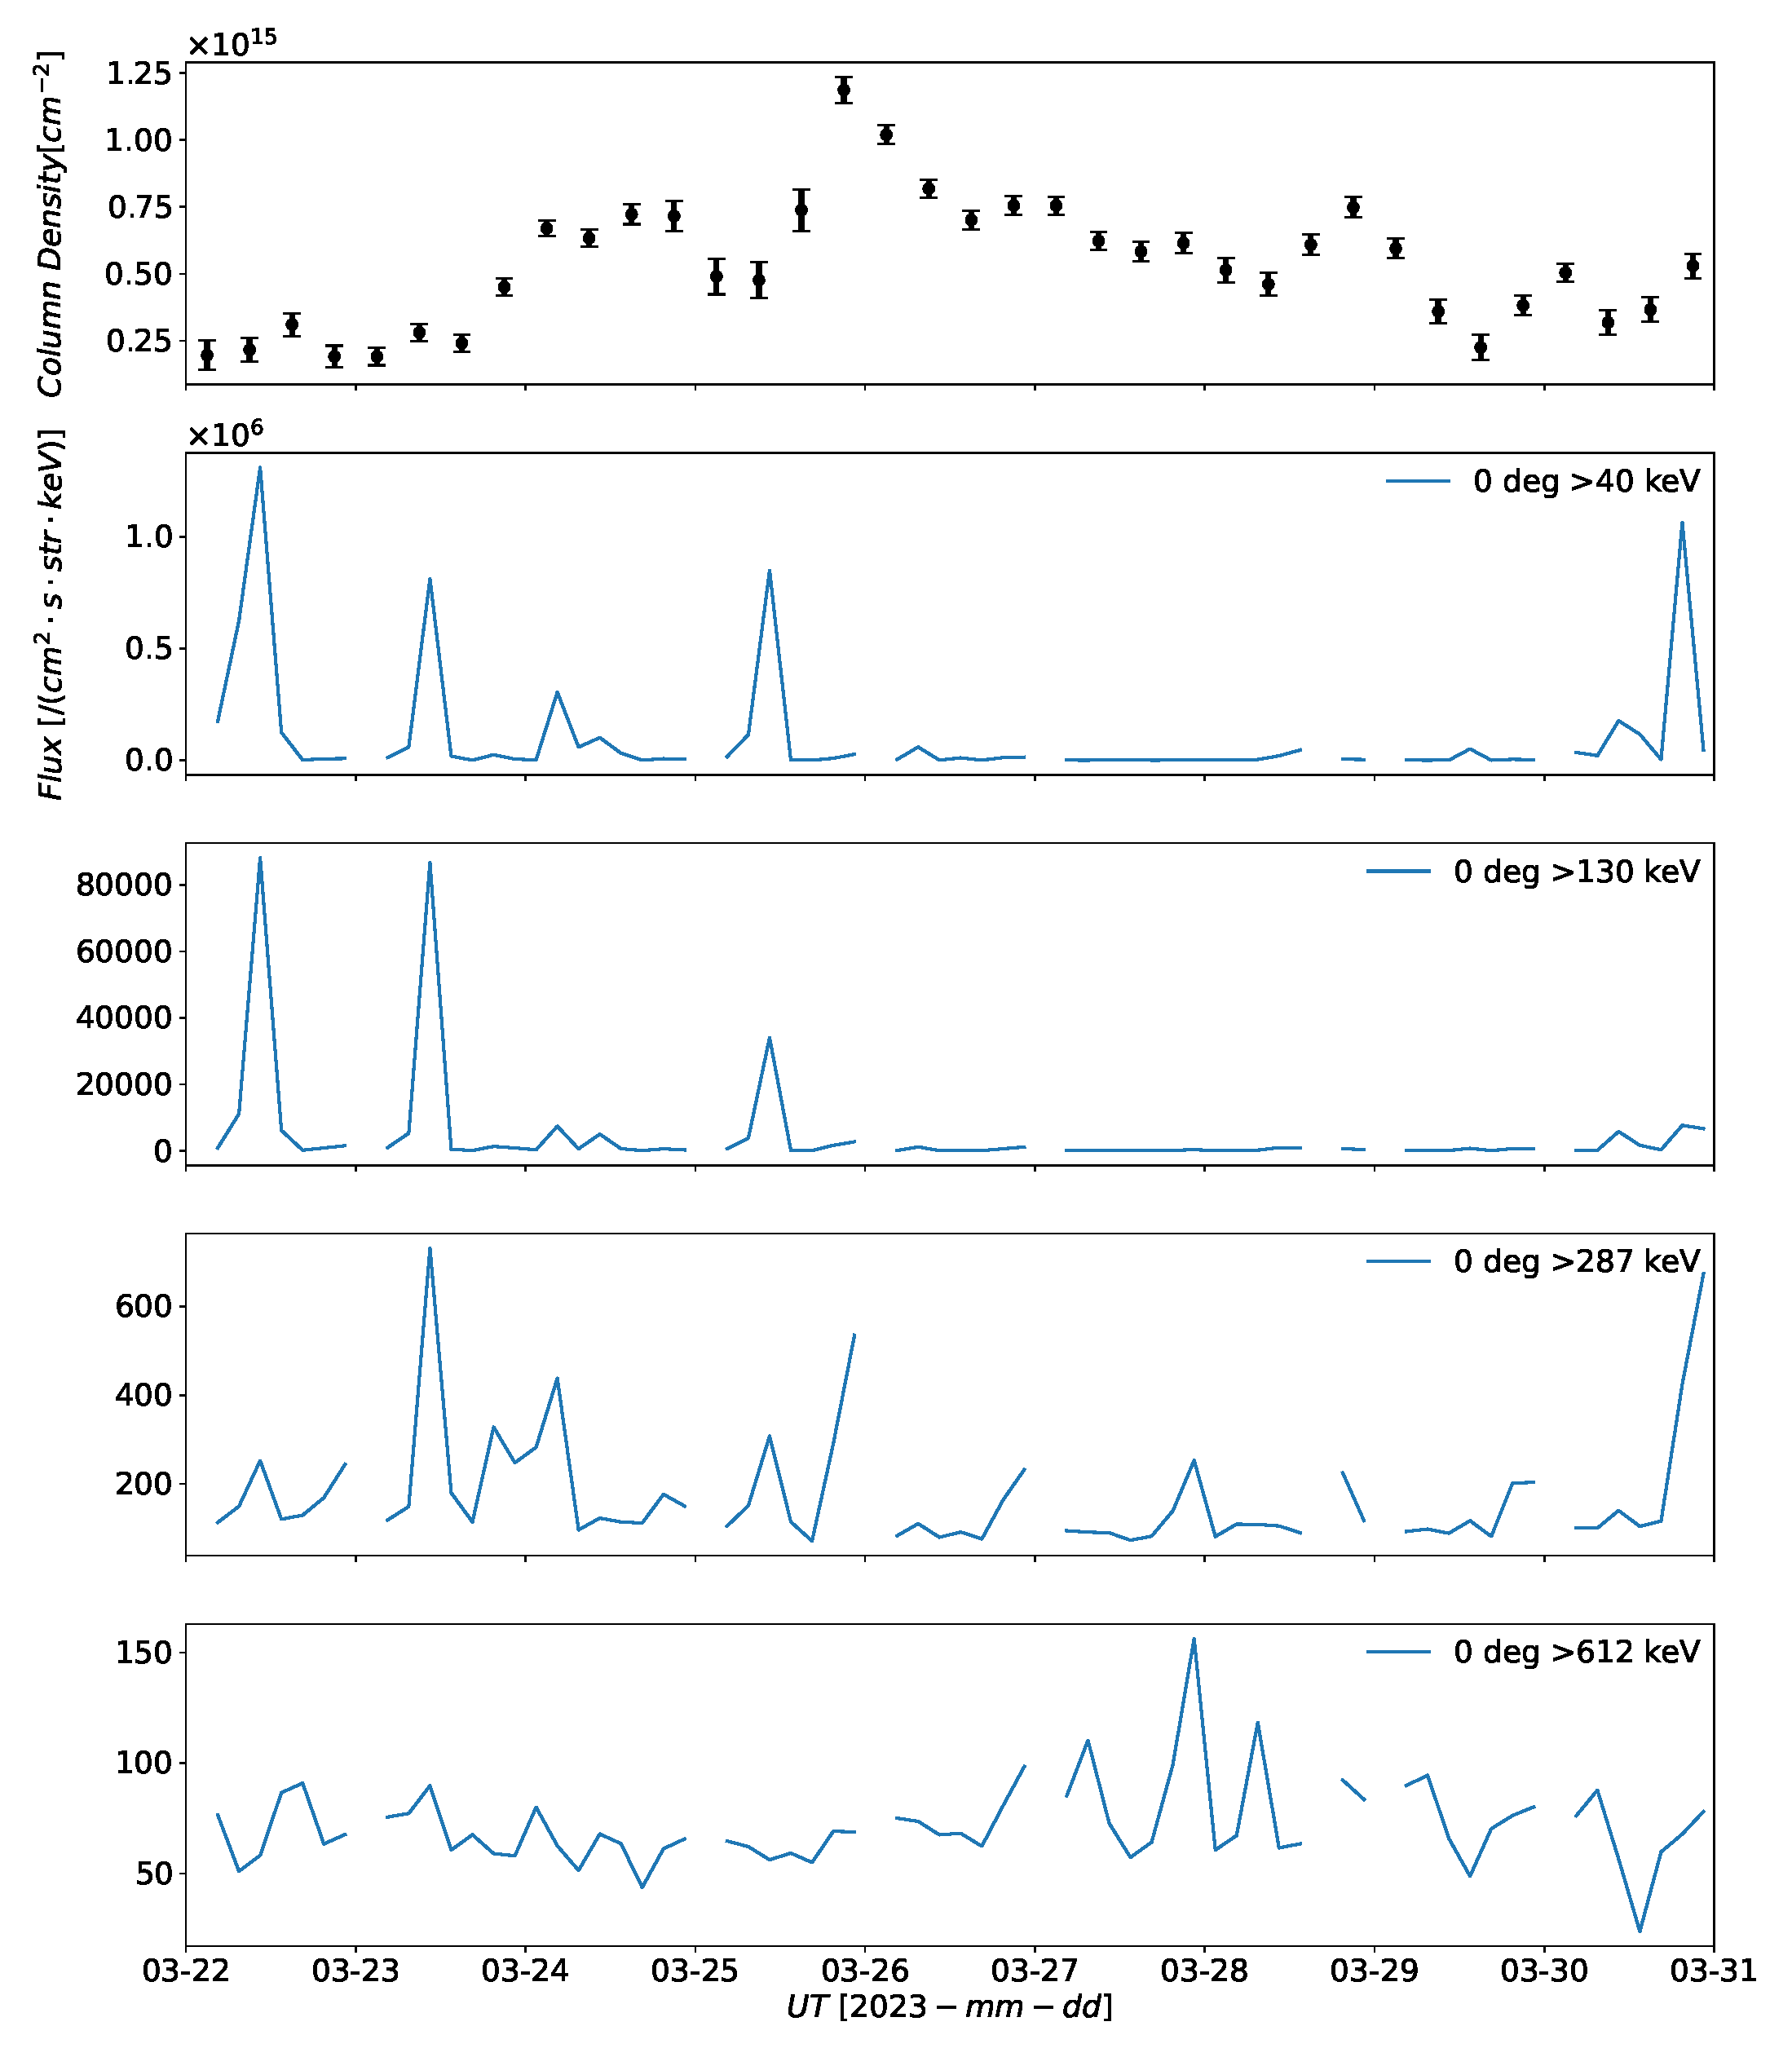
\includegraphics[width=\linewidth]{master_thesis_contents/master_thesis_fig/column_density_spectr6_poes0deg_syowa.pdf}
    \caption{昭和基地における柱密度(1段目。図\ref{fig:column_density_spectr6_syowa}と同じ)と電子フラックスデータ(2-5段目)との比較}
    \label{fig:ele_mmcd_syowa}
\end{figure}
\begin{figure}[htbp]
    \centering
    \begin{minipage}{\linewidth}
        \centering
        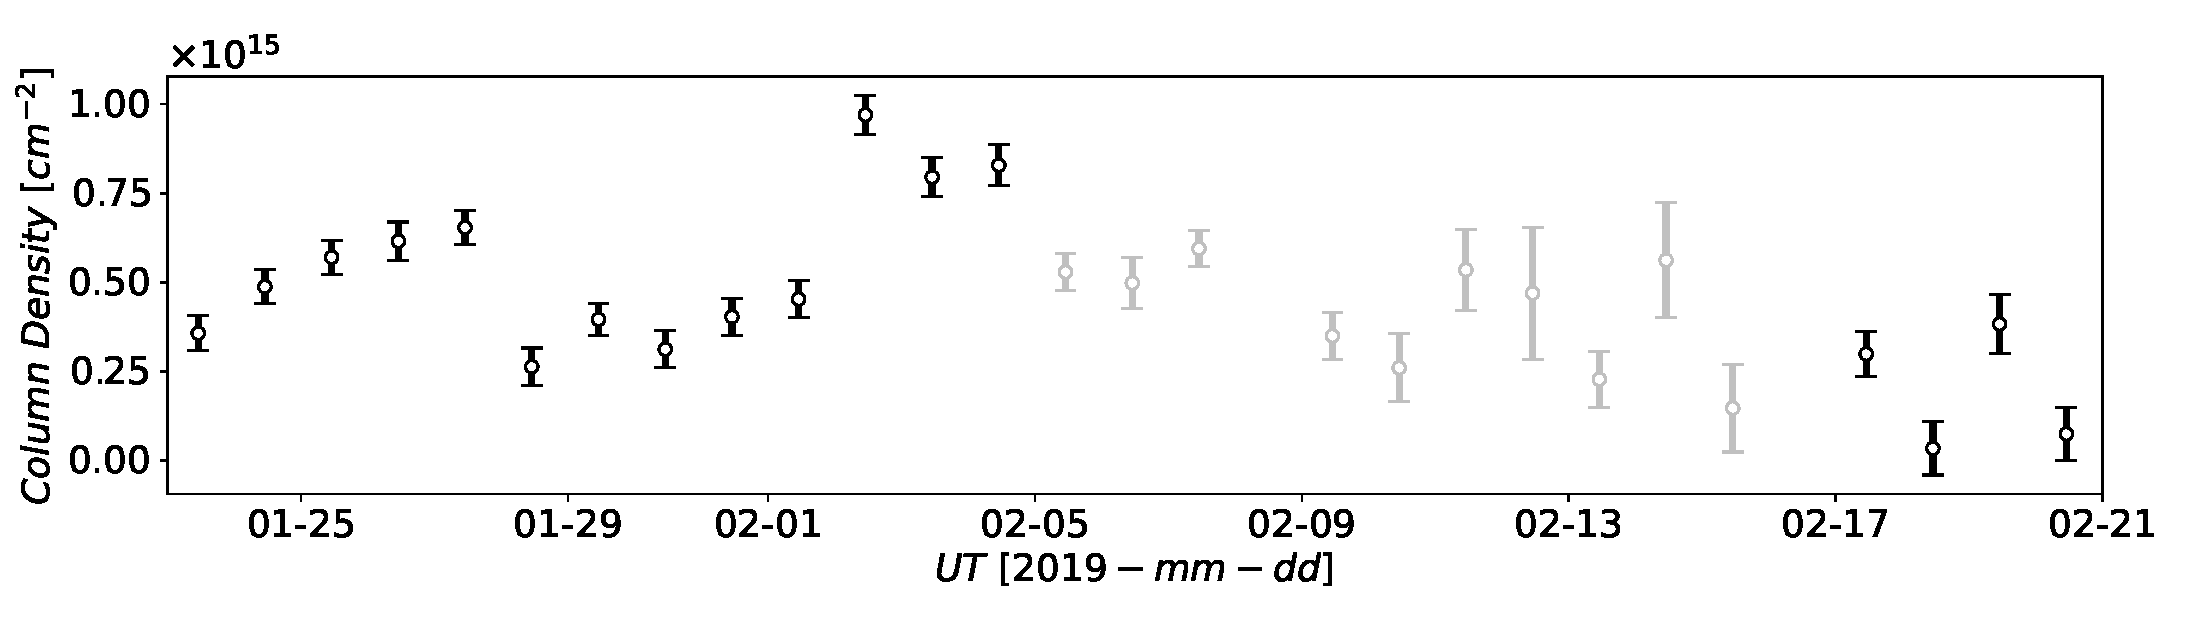
\includegraphics[width=\linewidth]{master_thesis_contents/master_thesis_fig/avg_ColumnDensity_tromsoe.pdf}
    \end{minipage}
    \begin{minipage}{\linewidth}
        \centering
        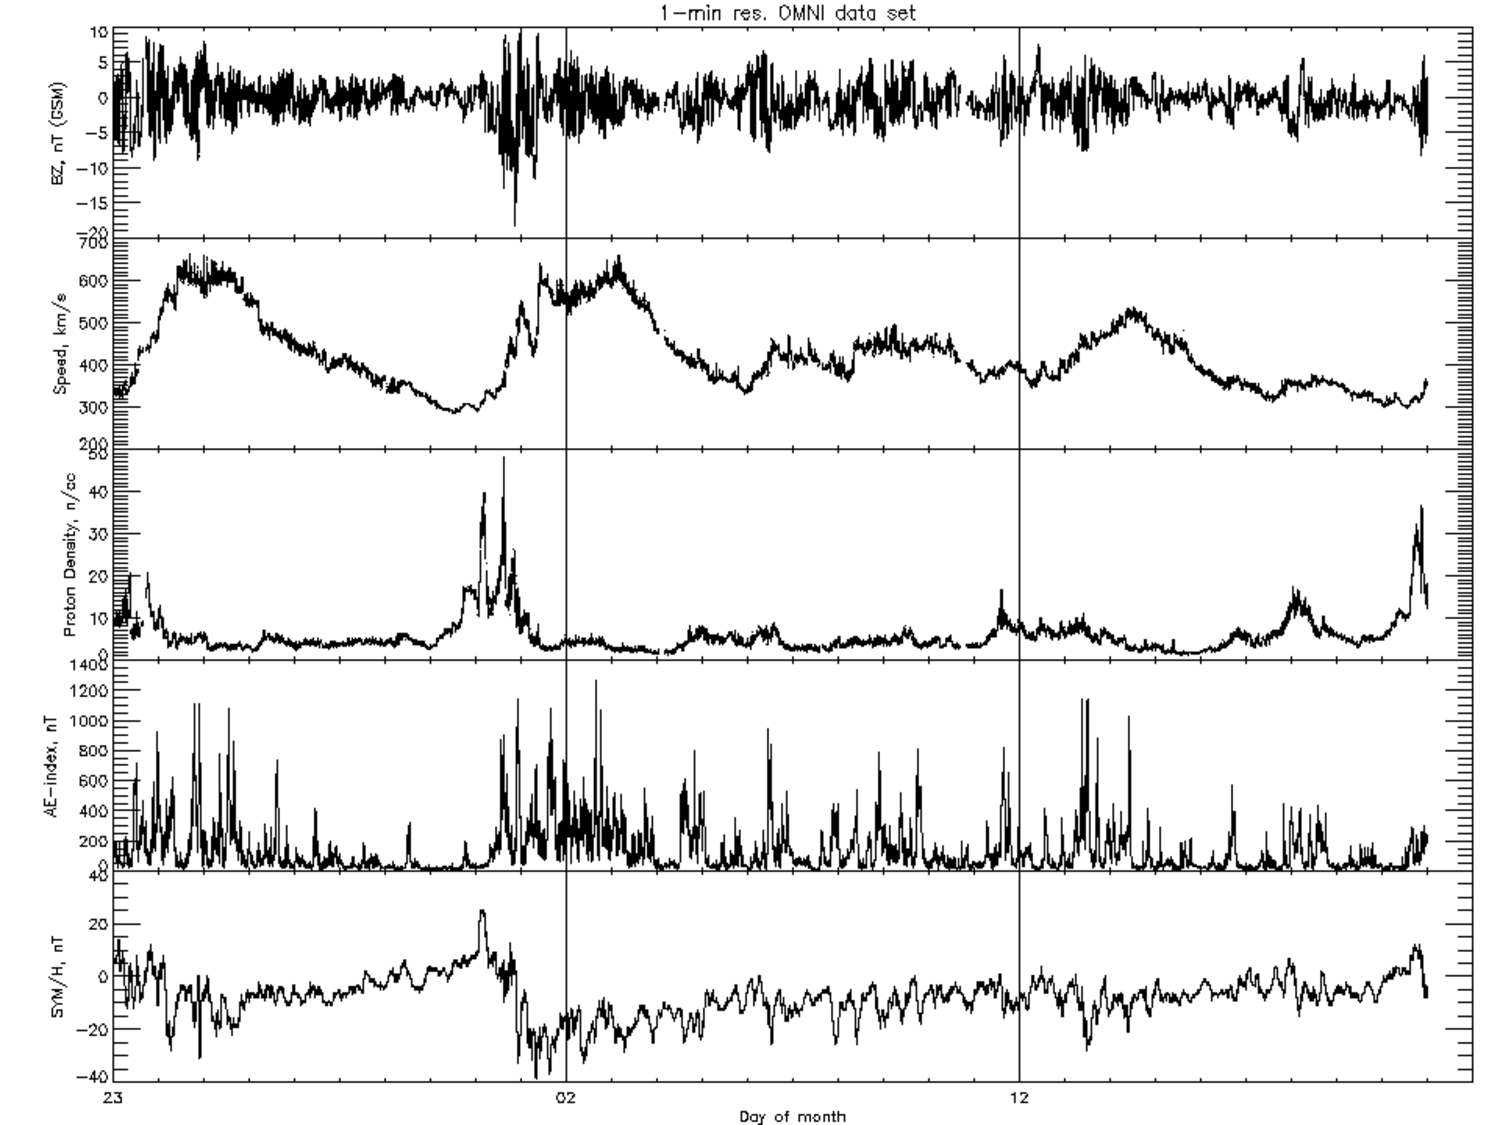
\includegraphics[width=\linewidth]{master_thesis_contents/master_thesis_fig/omni_tromsoe.pdf}
    \end{minipage}
    \caption{トロムソにおける柱密度(1段目。図\ref{fig:avg_ColumnDensity_tromsoe}と同じ)とOMNIデータ(2段目:地球磁場の南北成分、3段目:太陽風の速度、4段目:プロトン密度、5段目:AE指数、6段目:SYM/H)との比較}
    \label{fig:omni_mmcd_tromsoe}
\end{figure}
% 2つの図を整えて、揃えて出力する必要がある
% OMNIデータのAppendixを作る必要あり。
% SYM/HについてDst指数との関係を述べる。
\begin{figure}[htbp]
    \centering
    \begin{minipage}{\linewidth}
        \centering
        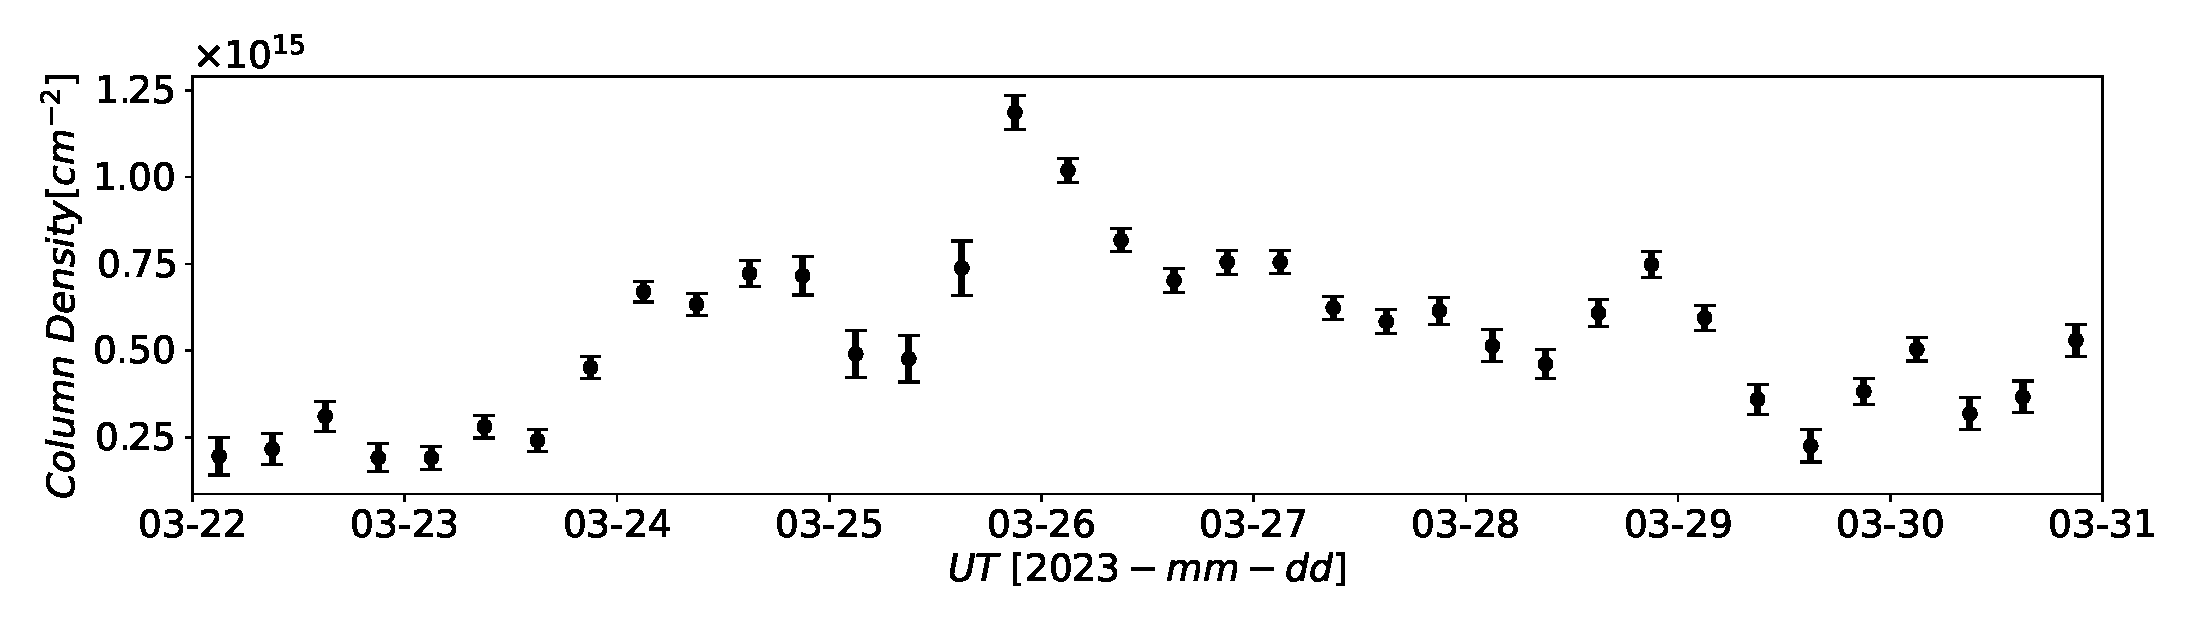
\includegraphics[width=\linewidth]{master_thesis_contents/master_thesis_fig/column_density_spectr6_syowa.pdf}
    \end{minipage}
    \begin{minipage}{0.96\linewidth}
        \centering
        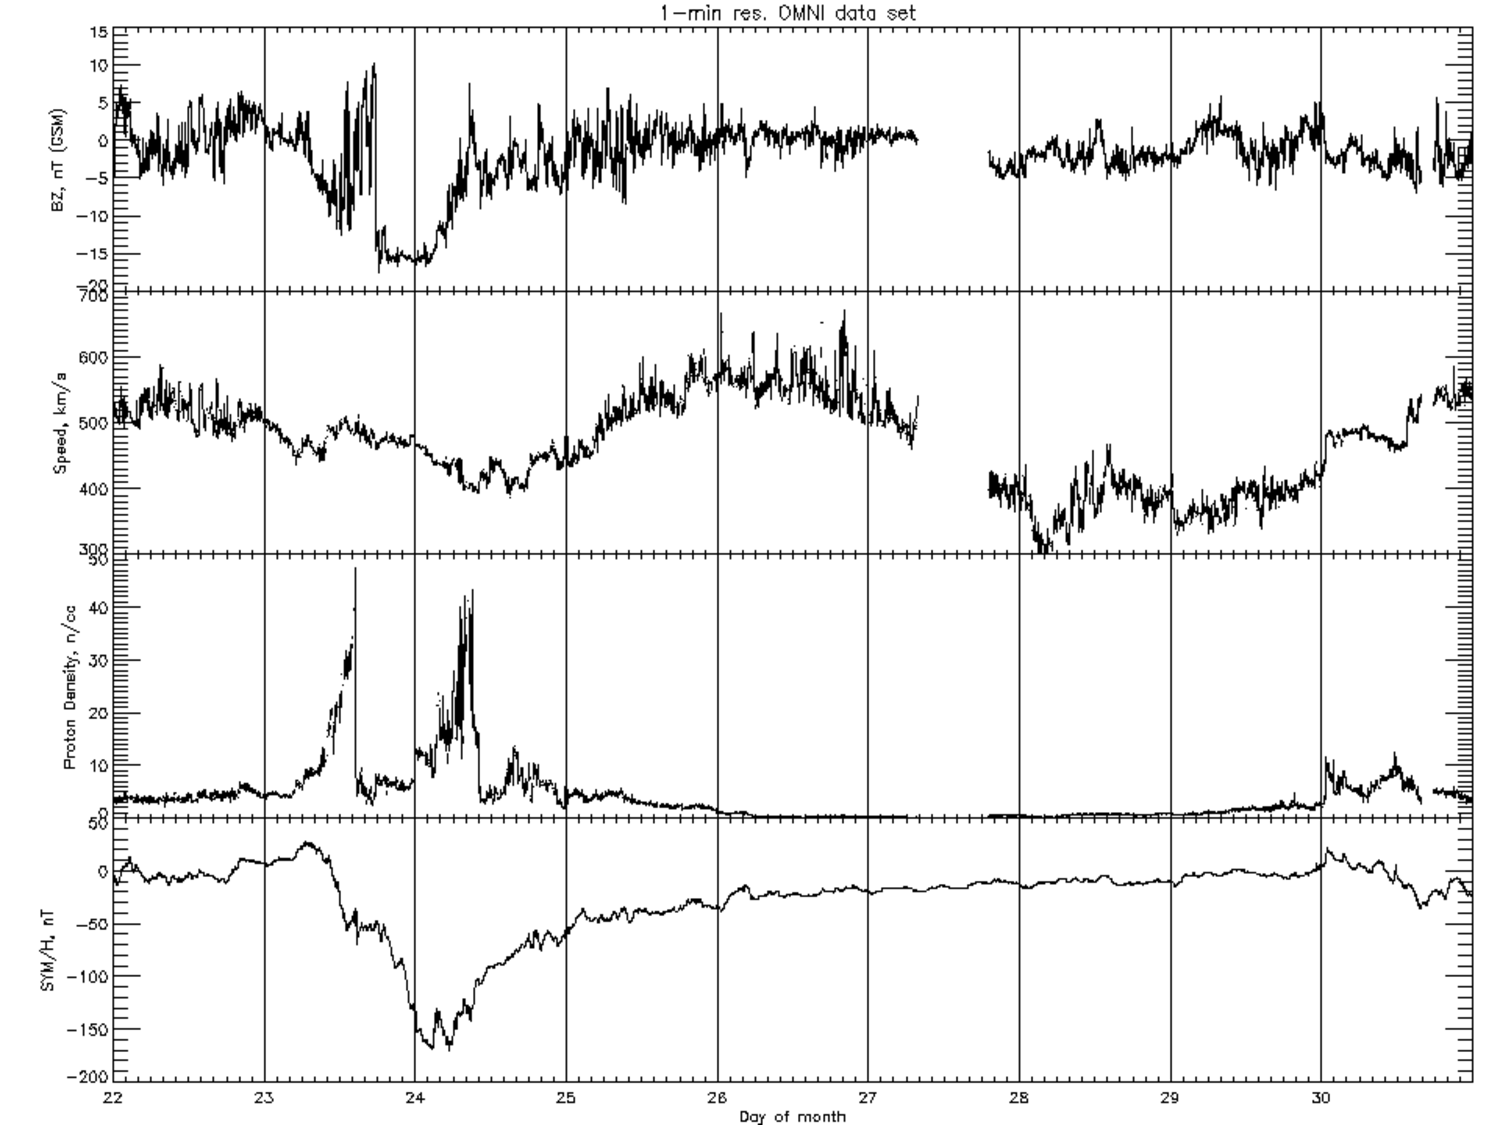
\includegraphics[width=\linewidth]{master_thesis_contents/master_thesis_fig/omni_syowa.pdf}
    \end{minipage}
    \caption{昭和基地における柱密度(1段目。図\ref{fig:avg_ColumnDensity_tromsoe}と同じ)とOMNIデータ(2段目:地球磁場の南北成分、3段目:太陽風の速度、4段目:プロトン密度、5段目:SYM/H)との比較}
    \label{fig:omni_mmcd_syowa}
\end{figure}
% 2つの図を整えて、揃えて出力する必要がある
% AE指数がない理由を述べる。
